This chapter covers the architecture and design of the system.
\section{General architecture}
In this section the general architecture of the \gls{theresa} system is described.
The idea for the new system is to reuse the concept of the already existing sampling system \gls{kapture}, which is using four \glspl{adc}, and expanding it to 16. Therefore, also the architecture of the latter is explained briefly.

\newpage
\subsection{New System THERESA}
In principle, the new system has the same structure, as \gls{kapture}. Notable differences are firstly the number of \glspl{adc}, which is increased up to 16. Secondly, the latter are not located on the daughter card anymore, but inside the Xilinx Zynq UltraScale+ RFSoC ZU49DR on the ZCU216 Evaluation Kit on which the front-end card is mounted.
%todo On THE xyz board? do we know what this is at this point?





\subsection{Requirements}





\paragraph{Data Rate}

ADC samples \@ \SI{2.5}{\giga \hertz} with 14-bit resolution.

\paragraph{Visualization/GUI}
\newpage
\section{Design of the front-end card}
In this section, the design of the front-end card is covered.



\newpage
\section{PCB-Layout}


  
\newpage
\section{Firmware}
\subsection{General Design}
\subsubsection{Firmware for Front-End Card}
\paragraph{Clocking}
\paragraph{SPI-Interface}
\subsubsection{Data Capture}
\begin{figure}[H]
	\centering
	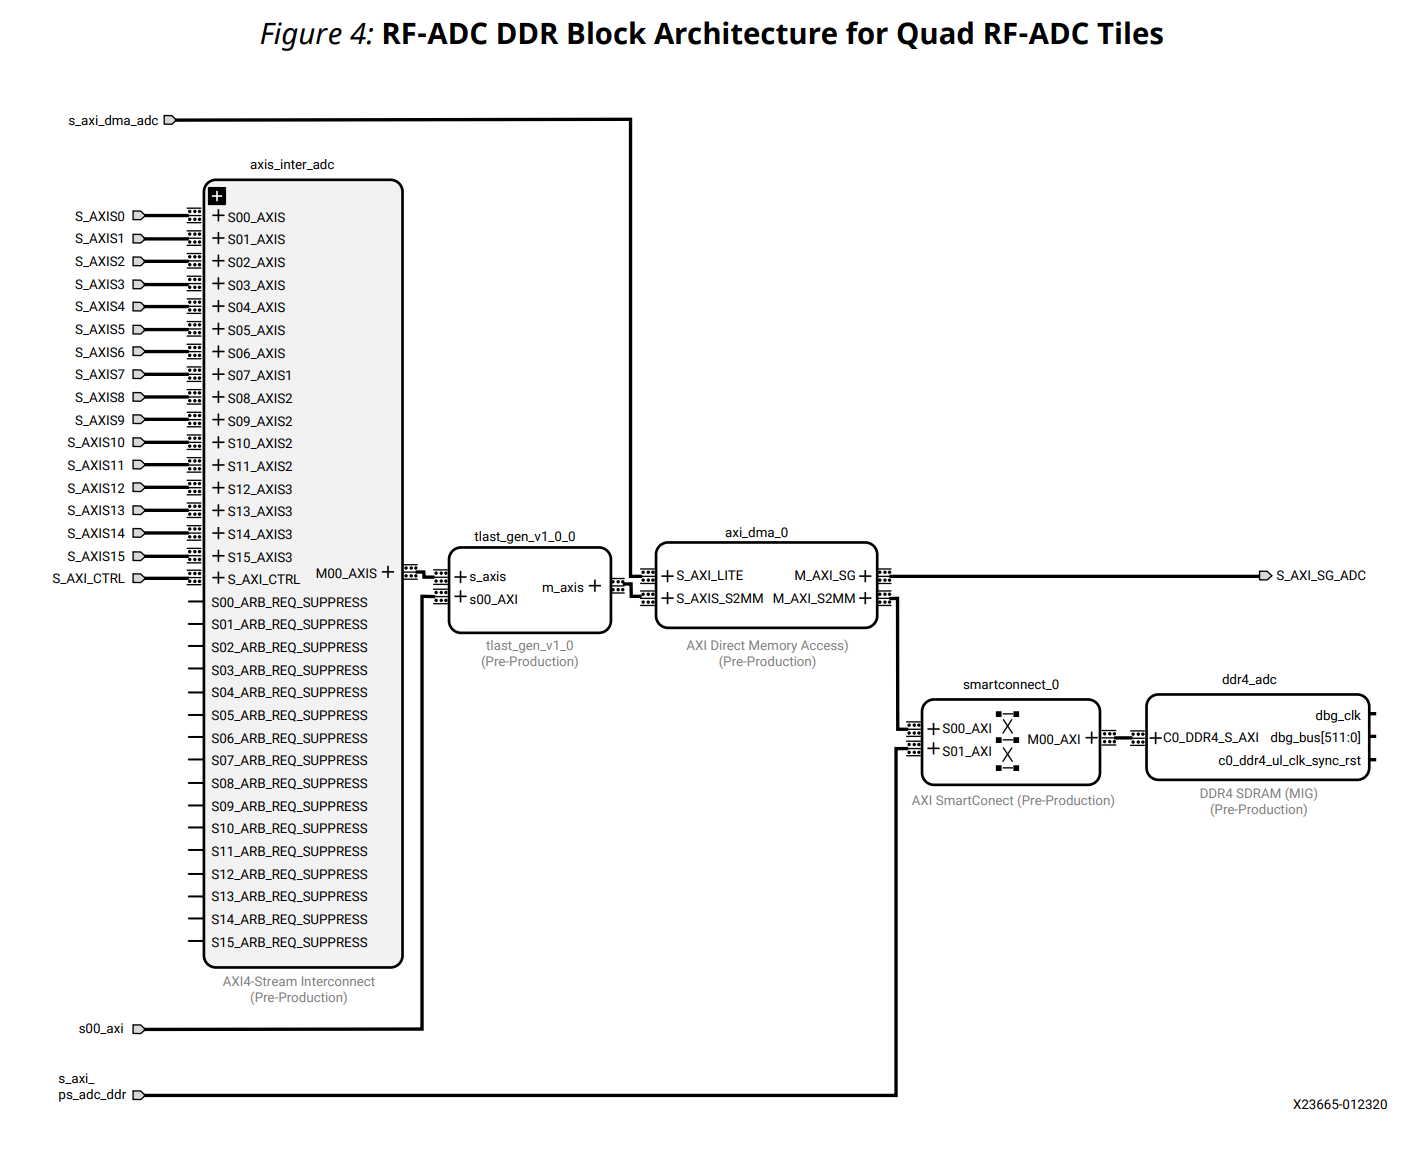
\includegraphics[width = 0.8\textwidth]{chap/04-work/img/adc_cap}
	\caption{Placeholder}
	\label{fig:adccap}
\end{figure}

\subsubsection{Visualization}





